\documentclass[11pt, a4paper, twocolumn]{article}
\usepackage[utf8]{inputenc}
\usepackage{multicol}
\usepackage{fancyhdr}
\usepackage{setspace}
\usepackage{indentfirst}
\usepackage{amsmath}
\usepackage{graphicx}
\usepackage{caption}
\captionsetup[table]{singlelinecheck=false}
\usepackage[subrefformat=parens,labelformat=parens]{subcaption}
\usepackage[a4paper]{geometry}
\geometry{top=1.95cm, bottom=1.8cm, left=2.4cm, right=2.4cm, headsep=0.5cm, headheight=1cm, 
            footskip=0in, footnotesep=0in, marginparwidth = 0pt,https://www.overleaf.com/project/625ab9c4557e178ba2f7d82c
            hoffset=0in, voffset=0cm}
\setlength{\parskip}{0cm}
\renewcommand{\baselinestretch}{1} 
\usepackage{hyperref}
\usepackage[backend=bibtex,style=numeric-comp,sorting=none,firstinits=true,maxbibnames=99]{biblatex}
\DeclareNameAlias{author}{last-first}
\bibliography{reference}


\pagestyle{fancy}
\renewcommand{\headrulewidth}{0pt}
\fancyhf{}
\chead{\footnotesize{}}
\rfoot{\thepage}

\usepackage{sectsty} 
\sectionfont{\fontsize{12}{15}\selectfont}
\subsectionfont{\fontsize{12}{15}\selectfont}


\usepackage{lipsum}  

\makeatletter
\renewcommand{\maketitle}{\bgroup\setlength{\parindent}{0pt}
\begin{flushleft}
  \onehalfspacing
  \fontsize{20}{23}\selectfont
  \textbf{\@title} \\
  \hfill \break
  \fontsize{12}{15}\selectfont
  \@author
\end{flushleft}\egroup
}
\makeatother

\title{End-to-end NP enrichment model}
\author{%
        \textbf{Ran Raboh}\\
        \fontsize{11}{14}\selectfont
        }

\begin{document}

\twocolumn[
  \begin{@twocolumnfalse}
    \maketitle

\noindent \textbf{Abstract.} Text-based NP enrichment is a task that aims at evaluating the relation between noun phrases in the text that can be expressed as a preposition. The paper proposes an end-to-end architecture for evaluating the relation between NP span pairs. The proposed architecture incorporates effective novel techniques ranging from graph neural networks to a span encoding strategy which effectively captures information about the spans in the document.
The code is available at \url{https://github.com/ranraboh/TNE\_TASK}

\noindent \textbf{Keywords:} Text-based np enrichment, Tne, Graph neural network, Coreference resolution.

  \end{@twocolumnfalse}
  \vspace{1.5em}
]
% \begin{multicols}{2}

\section{Introduction}
\label{introduction}
Text-based NP enrichment is a task that aims at evaluating the relation between noun phrases in the text that can be expressed as a preposition.
TNE is a promising task that can be applied to a variety of natural language pipelines to improve the performance of many NLP tasks.
The core idea is to enrich each noun phrase by providing further information regarding the relation it holds to other mentions in the text. higher-rank NLP tasks can leverage the information recovered by the NP enrichment task to improve text comprehension skills and achieve higher results.
Mastering this skill is a major step toward analyzing and understanding the meaning of the text.
The paper sets two main goals: (1) build an end-to-end NP enrichment model which exceeds the performance of the baseline model.
(2) Analyze the impact of the co-reference cluster's external knowledge over the TNE task. The paper aims to leverage the knowledge about the co-reference relations of the NP spans and examine the extent to which the results have been improved. 
The model assumes that the co-reference clusters between the NP spans are given as input under the assumption that a state-of-the-art model's ability to unravel the co-reference relations can be used in lieu to the provided information in a way that will not significantly affect the outcomes.

\section{Text-based NP enrichment}
\label{task}

Text-based NP enrichment task proposed in \cite{tne}. The objective of the task is to detect the relations between NP spans in the text. The task focus on relations that can be described as prepositions such as for, in, against, etc.
The relations can be explicit as in "The book is 
\underline{on} the coffee table" where the preposition connection is fully expressed and stated outright or it may be implicit where the reader needs to fill in the gaps and make inferences based on the context. the implicit links are more challenging to infer.
An example of implicit relation can be found in the following sentence:
'I found the book under my bed, the pages were torn on the desk'.
based on the context readers can infer that the pages are of the book. That is, the relation that holds between the term 'pages' to the noun phrase 'the book' is best described by the proposition 'of'.

A TNE model receives a text, and a list of the NP spans which are denoted by their first and last positions in the document and should determine for each NP pair the connecting preposition or NONE in case no relation holds between the compared mentions.
Figure 1 demonstrates a document that appears in the data set. 

\begin{figure}
    \centering
    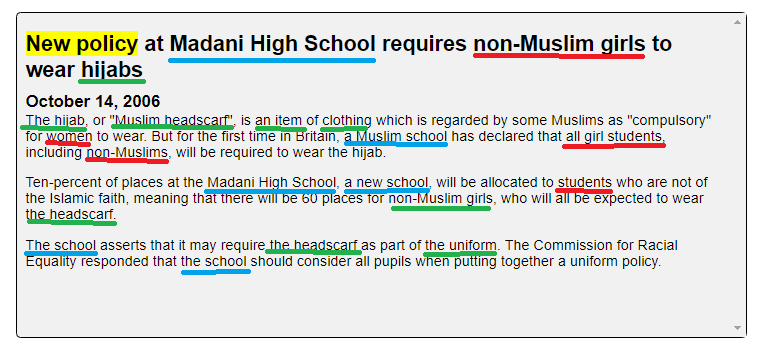
\includegraphics[width=\linewidth]{sample1.png}
    \caption{a document from the dataset. the document used to demonstrate relations between noun phrases and show how the expression 'new policy' relate to other NP spans in the document using different type of prepositions.
    the expressions which refers to it using preposition of 'at' are underlined with blue line. relations of 'about' marked with green while relations of 'for' preposition marked with red.  }
    \label{fig:my_label}
\end{figure}

\underline{Task definition:} Given a sequence of noun phrases $\mathbf{n}_1$, $\mathbf{n}_2$.., $\mathbf{n}_k$ that appeared in the text and set of prepositions $\mathbf{p}_1$, $\mathbf{p}_2$, ..., $\mathbf{p}_m$.
for each ordered pair of noun phrases ($\mathbf{n}_i$, $\mathbf{n}_j$) determine the preposition $\mathbf{p}_t$ which best describes the relation between $\mathbf{n}_i$ to $\mathbf{n}_j$ or declare that no relation holds between them.

The input of the model composed of:
1) the content of the document as a set of tokens $\mathbf{w}_1$, $\mathbf{w}_2$, ..., $\mathbf{w}_n$.
2) an ordered list of NP mentions N = [$\mathbf{n}_1$, $\mathbf{n}_2$.., $\mathbf{n}_k$]
3) set of coreference clusters C = [$\mathbf{c}_1$, $\mathbf{c}_2$,.., $\mathbf{c}_r$] where cluster $\mathbf{c}_i$  $\mathbf{\subseteq}$ N is non empty list of NP mentions. 


The output is a set of triplets of the form ($\mathbf{n}_i$, prep, $\mathbf{n}_j$) such that i $\mathbf{\neq}$ j.
$\mathbf{n}_i$, $\mathbf{n}_j$ are noun phrases that appear in the text where the first is referred as an anchor and the last is named complement and prep is the predicted relation between them or NONE.


\section{Prior work}
\label{priorwork}

The paper Text-based NP enrichment \cite{tne} introduced the baseline model. 
The baseline model uses Span Bert transformer-based encoder which maps each span to a contextual embedding.
Span Bert \cite{joshi2019spanbert} is a pretrained language that is built upon Bert \cite{devlin2018bert} and used to learn a representation of the spans based on their context. Span Bert is renowned to be highly effective and perform well on span-based tasks.
The span representation is fed into two MLPs which encode the span as an anchor and complement.
The model then concatenates each pair of anchor and complement and passes it into a prediction multi-class classifier that computes probabilities over the preposition labels.

The paper presented two variants: the decoupled variant in which the prediction is a two-step process a binary decision that detects if the NPs are linked followed by a multi-class classifier used to determine the corresponding preposition.
the coupled variant has only a single multi-class head that outputs the connecting preposition or NONE, in case the NPs are not connected.

\section{Graph methods}
\label{graphmethods}

GNNs (which were first introduced at \cite{gnn}) are a class of techniques and methods designed to perform on graph-structured data and have shown strong performance on many NLP tasks \cite{gnnfonlp}. GNNs models compose of multiple graph convolution layers stacking on each other. The graph convolution operator considers the immediate local neighborhood of each node and uses that information to further update the node's features.
The model incorporates GNNs to learn a more informative representation for each span.
There are two major categories of graph techniques. 
(1) static method where the graph is constructed during pre-processing phase using external knowledge.
(2) dynamic method where the graph structure is dynamically learned during the training phase.

\subsection{Coreference graph}
\label{coreferencegraph}

The idea is to exploit the external knowledge regarding the co-reference clusters to get a richer representation.
Co-reference clusters are a partition of the noun phrases in the document into disjoint classes C = [$\mathbf{c}_1$, $\mathbf{c}_2$,.., $\mathbf{c}_r$]
such that each class $\mathbf{c}_i$  $\mathbf{\subseteq}$ N contains a non-empty set of expressions that refer to the same entity where N is a set of the NP spans in the text. We state that two phrases are co-referent to each other if they belong to the same co-reference cluster.
The information can be easily described as a graph in the following manner:
Let's denote an undirected graph G = (V, E) such that the nodes are the NP spans in the text. two nodes are connected by an edge if and only if the corresponding spans are co-referent to each other. Adding to that, edges that connect each node to itself.

The co-reference knowledge can be leveraged to make the noun phrases to be more clear and understandable. The expressions might be (1) ambiguous, for instance, the term 'page' can be a sheet of paper or a name of a person. Clarifying it can positively affect the predicted relation to other NP spans in the text.
(2) lacked of informative details, that is, the phrase does not contain clear and full details on the entity it refers to, e.g. references to an entity that has been previously introduced in the text. 
Applying the GNN model on the co-reference graph is a popular technique that is used in a wide range of NLP applications (as \cite{corefsummarizartion} \cite{entitymentions}). Each node gains a representation that is mindful of itself and the node's direct neighborhood in the graph.
The NP companions that belong to the same cluster share information to reconstruct a representation that is more informative, clear, comprehensible, and self-contained.

\subsection{Dynamic graph}
\label{dynamicgraph}

Dynamic graph-based methods have been successfully used in a variety of NLP tasks. as opposed to static graph construction where the graph topology is a prior knowledge provided by the information expert which is presumed to be indispensable for the decision. In the dynamic graph paradigm (as introduced and used in \cite{dynamicgraph} \cite{dynamicgraphframeowrk}), the graph interactions are not set manually but learned by the model. dynamic graph paradigms are designed to learn the graph structure and implicit links to effectively share the information between the nodes.
The motivation is to share information among spans to absorb vital information that might be crucial to determine the relation between NP pairs.
Let's denote a directed graph G = (V, E) where the vertices are the spans in the document and the edges are dynamically evaluated by the model.
for each edge e = ($\mathbf{v}_x$, $\mathbf{v}_y$) denoted by its endpoints spans, the model computes a score that measures the importance to capture the information of $\mathbf{v}_y$ in the representation of $\mathbf{v}_x$ node,
such that spans that positively improve the encoding of other entities will get a higher score. The operator then aggregates the information according to the learned weights.

\textbf{Enforce sparse graph}: The naive approach of the dynamic paradigm is to learn a fully-connected adjacency matrix. The naive approach has a major flaw in which the model learns noisy information due to ineffective aggregation over unrelated neighbors. The dynamic graph module enforces the model to extract a sparse graph with a small number of connections. The intuition is that naturally each NP span is influenced by only a few entities in the text. The sparsity mechanism that I came up with is as follows:
A score is assigned for all possible pairwise combinations of spans in the document.
The evaluated scores are normalized with zero mean and unit variance. scores that their standard deviations are 1.5 above or -1.5 below the mean are modeled in the graph and the others are left out and do not include in the aggregation process.

This procedure guarantees that approximately 85\% of the values lie within 1.5 standard derivations of the mean and considers 15\% of the spans when constructing the graph. According to the statistics reported by the NP enrichment task paper \cite{tne}, a typical document in the data-set has an average of 38 noun phrases. Hence, each node will be connected to 5 neighbors on average.

\section{Architecture}
\label{architecture}

This section presents an overview of the components of the model. The architecture is divided into two main components: (1) the frontend which is responsible to learn representation for each span in the text (2) the backend, which given a representation of the spans, produces probabilities for triplets of anchor \& complement NP spans and a preposition. That is, the backend evaluates how likely the relation between a pair of NP spans is to be each one of the prepositions. Figures 2, and 3 illustrate the architectural components of the model.

\begin{figure}
    \centering
    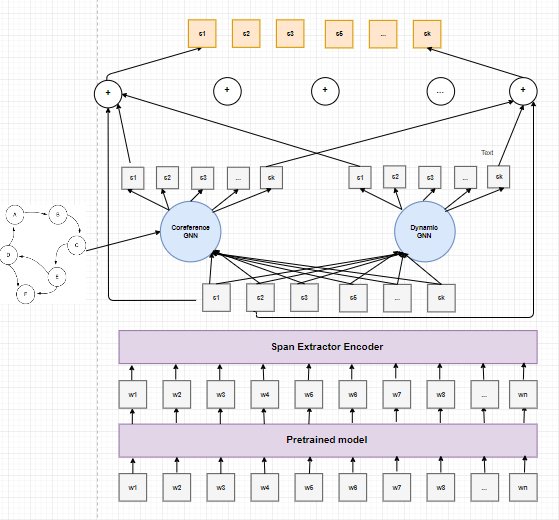
\includegraphics[width=\linewidth]{frontend.png}
    \caption{Frontend architecture which graphically depicts the stages to obtain representation for the spans in the document,   }
    \label{fig:my_label}
\end{figure}

\subsection{Pretrained model}
\label{pretrained}

Pre-trained language models are models that have been trained over large-scale data and acquired understanding capabilities which used to learn contextual encoding of the tokens in the text.
Deberta \cite{he2021debertav3} is a popular pre-trained architecture that is built upon BERT \cite{devlin2018bert} which used two primary techniques to enhance its performance: 
(1) disentangled attention mechanism which treats the content and position of each token separately using disentangled matrices.
(2) scale-invariant fine-tuning which incorporates adversarial training examples to improve the model robustness and generalization.

There is a wide range of pre-trained models that have been introduced. Among the competitors that have been tested, the Deberta model yields the highest results and was adopted to be part of the pipeline of the model. Despite that Span Bert is renowned to work well with span-based tasks, the fact that the spans are given in advance drives us to select a token-wise pre-trained method and extend it to learn representation for the spans in the document.

The initial step is to apply Deberta to assign each token a representation based on its context.
Deberta considers the individual tokens and the next step is to reconstruct the word spans. 


\subsection{Span extraction encoder}
\label{spanencoder}

The model uses two additional tokens which appear at the beginning and end of each span in the text. 
The new tokens are used to capture span-level information.
After obtaining contextual embeddings of the tokens, the data is passed into the span extractor module. 
The module hierarchically refines the encoding of the tokens to gain a better representation. The first layer considers a large margin window around the spans. The window gradually shrinks through including a local neighborhood around the span until it just contains the inner tokens of the span. The transformer-based pre-trained model weighting the significance of each token at each step and aggregates the information regarding the tokens according to the learned scores. The aggregation is done over the entire set of tokens and on top of that is inherently order-invariant (although positional embedding technique has been adopted) which makes it susceptible to convey noisy data. The motivation for the encoder technique is that it applies to shorter sub-sequences to refine the encoding of the tokens, carefully wipe out the noise and gently propagate information from different parts of the text.
The representation gained by the hierarchical encoder adds up to the encoding acquired by the pre-trained layer. 

Each span is assigned with an initial representation as the following ($\mathbf{x}_1$, $\mathbf{x}_2$)
where $\mathbf{x}_1$ is the encoding of the start and end tokens obtained by the pre-trained model while, 
$\mathbf{x}_2$ is the encoding of the start and end tokens after applying the hierarchical encoder.

\subsection{Graph-based methods}
\label{graphbasedmethods}

Section \ref{graphmethods} presents the Graph neural network and graph-based components which are integrated into the text-based enrichment model.
The initial step computes a representation for each span which is denoted by ($\mathbf{x}_1$, $\mathbf{x}_2$).
The graph-based methods are used to extract further information which adds up to the initial encoding to get a richer representation.

\textbf{Coreference graph:} The goal is to leverage the external data regarding co-reference clusters to add up essential information that leads to a more informative, clear, and self-contained representation.
The graph is constructed during the pre-processing phase and given as input for the model. The graph neural network produces a representation for the spans that is mindful of the co-reference clusters and beneficial for evaluating the correct preposition relations between NPs in the text.

\textbf{Dynamic graph technique:} Dynamic graph neural network is employed to learn the connections which map out the way the information is conveyed between the spans. The goal is to enrich the initial representation with valuable information that is shared among the spans to improve the predictive ability of the model.
A sparsity scheme is applied to the learned graph structure to enforce that each span can be influenced only by a small number of entities.

The enhanced representation for the spans is denoted as ($\mathbf{x}_1$, $\mathbf{x}_2$, $\mathbf{x}_3$, $\mathbf{x}_4$) where
$\mathbf{x}_3$ is the information extracted from the co-reference graph and $\mathbf{x}_4$ is the encoding obtained by applying the dynamic graph neural network model.

\subsection{Prediction layer}
\label{predictionlayer}

After obtaining representations of the spans in the document. The model used MLPs to encode each span as an anchor and complement.
Each pair of anchor and complement is fed into a prediction model along with the relative distance between them. The relative distance is a piece of information that is injected into the model and presumed to be vital to account for when making a prediction. The prediction layer produces probabilities for triplets of anchor \& complement NP spans and a preposition. That is, the prediction layer evaluates how likely the relation between a pair of NP spans is to be each one of the prepositions labels.

\begin{figure}
    \centering
    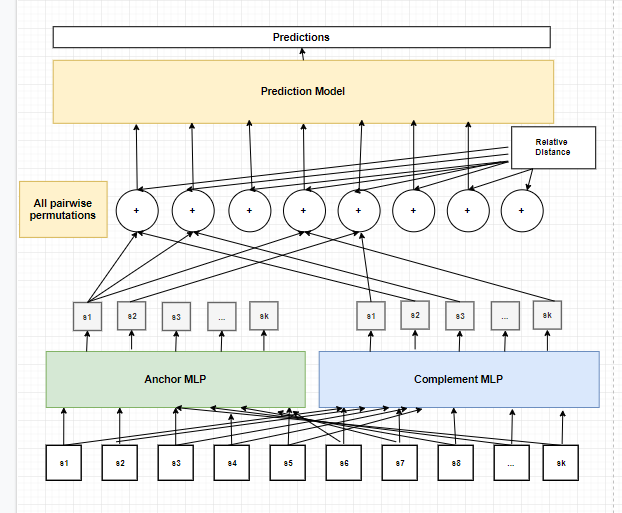
\includegraphics[width=\linewidth]{backend.png}
    \caption{Backend architecture which graphically depicts the steps to produce the probabilities for each pair of spans.    }
    \label{fig:my_label}
\end{figure}


\subsection{Notations}
\label{notations}

The frontend stage output encoding $\mathbf{q}_1$, $\mathbf{q}_2$.., $\mathbf{q}_k$.
The backend takes the representation of the spans and encode each span as an anchor and complement using MLP model which denoted as $\mathbf{q}_i^{anchor}$ and $\mathbf{q}_i^{comp}$ respectively. 
\begin{gather}
    q_i^{anchor} = MLP_{anchor} (q_i) \\
    q_i^{comp} = MLP_{comp} (q_i)
\end{gather}

for each pair of NP spans ($\mathbf{n}_i$, $\mathbf{n}_j$), the model learns a distribution P over the list of preposition labels. The span pair scoring function s(i, j) is a MLP neural network over concatenation of
the encoding of span i as anchor $\mathbf{q}_i^{anchor}$, span j as a complement $\mathbf{q}_j^{comp}$ and the relative distance between them $\mathbf{\phi}$(i, j).
\begin{equation} \label{eq:04}
    s(i, j) = MLP_{pred}(q_i^{anchor}, q_j^{comp}, \phi(i, j))
\end{equation}
Applying the softmax function turns the real-values scores into probabilities. The distribution P over the preposition list is computed as follows:
\begin{equation} \label{eq:04}
    P = \dfrac{e^{s(i, j)}}{\sum_{j'\in{N}} e^s(i, j')}
\end{equation}

\section{Imbalanced data}
\label{imbalanced}

Imbalanced data is a common issue in multi-class classification problems. Text-based enrichment is a case in point where the classes are not presented equally in the data set. an overwhelming majority (above 80\%) of the relations between pairs of spans is None which means that no relation holds between them.
When using the standard unweighted loss function, the training is not effective and the model is struggling to correctly predict low-frequency relations.
The unweighted cross entropy loss is defined as:
\begin{equation} \label{eq:01}
    CE = -\sum_{c=1}^{|P|} y_clog(\hat{y})
\end{equation}
where P is the number of labels and $\mathbf{y}_c$ is 0 or 1 indicating whether class label c is the correct classification.  

The weighted loss is used to tackle the imbalanced problem by weighting each class based on statistics over the training data. I've divided the preposition labels into four groups in conformity with the frequency they appeared in the training set. The first group contains the dominant label (NONE), the last group contains the labels that have the least number of occurrences in the data and the other labels are partitioned into the groups according to their frequency.

The groups are assigned with a constant coefficient ($\mathbf{g}_1$, $\mathbf{g}_2$, $\mathbf{g}_3$, $\mathbf{g}_4$) respectively.
In weighted cross-entropy, the loss term for each class is multiplied by the corresponding group multiplicative factor $\mathbf{g}_i$. 
Let's denote W = [$\mathbf{w}_1$, $\mathbf{w}_2$, ..., $\mathbf{w}_{|C|}$] to be the weights of the classes such that the weight of each class is the coefficient term of the group that the class belongs to.
The weighted loss entropy loss is defined as:F
\begin{equation} \label{eq:02}
    CE = -\sum_{c=1}^{|P|}w_c y_c log(\hat{y})
\end{equation}
The motivation is to assign a higher weight to the labels that appear more rarely in the training data to enhance their importance. A misprediction of infrequent classes has more impact on the loss value than an error in common classes.
Hence, the model is less likely to ignore small-size classes.

Another technique that has been used to tackle the imbalanced problem is periodically to include only the concrete relations between NP spans. In some probability, the training leaves off the pairs that no relation is held between them and keeps only the concrete relations. The empirical analysis has shown that this approach slightly improves the results.

\section{Evaluation metrics}

Following previous works, the metrics precision, recall, f1, and accuracy are computed over the preposition links and reported in Table \ref{tab:01}.
Additionally, the paper reports the results over the unlabeled links. A binary decision that evaluates for each pair of two mentions whether they are connected or not.

\begin{table}[t]
\caption{[Results] the metrics have been computed over the evaluation set. See section \ref{discussion} (Discussion) for more details}
\begin{tabular}{l c c c c}
\hline
model & p & r & f1 & a  \\
\hline
Coreference \\
enhanced & 0.651 & 0.525 & 0.581 & 0.879\\
model\\
Paper \\
standard & 0.642 & 0.519 & 0.574 & 0.865 \\
variant\\
Baseline\\
model  & 0.658 & 0.434 & 0.523 \\
\cite{tne}\\
\hline
\end{tabular}
\label{tab:01}
\end{table}

\section{Results \& Conclusions}
\label{conclusions}

The paper presents an end-to-end NP enrichment model. Two variants of the model have been evaluated: the coreference-enhanced variant which incorporates a graph-based component to augment the model base data with information about the co-reference chains and the standard variant that shares the same architecture but does not make use of the co-reference information.
Table \ref{tab:01} shows the results of the paper models.
Overall, the best model yielded results of 0.581 over f1, 0.651 precision, 0.525 recall, and 0.879 accuracy over the evaluation set.
The experimental results have shown that the co-reference cluster's data is valuable and improves the overall results. However, the improvement is not significant. My hypothesis based on the findings is that the model inherently tries to unravel the co-reference chains to perform well on the TNE task. Conceptually the model is liable to learn these interactions using components such as a transformer or dynamic graph neural network. As a consequence, the provided information slightly benefits the model to gain better results.

\section{Discussion}
\label{discussion}

The metrics that have been reported in the paper are evaluated over the development set. For the coreference-enhanced variant, the model is using the information regarding the co-reference clusters which are not part of the input on TNE task. Unfortunately, the predictions of the standard variant have yielded lower scores over the test set (which is on par with the baseline). Further investigation should be conducted to unravel the gap between the results on the evaluation set to the scores on the test set.

% \bibliographystyle{unsrt}
% \bibliography{reference}
\printbibliography



\end{document}
